\documentclass[11pt]{article}

% This line looks for the preamble in the folder "next door"
% It goes UP one level (..) then DOWN into (common)
% common/preamble.tex

% --- Page Setup ---
\usepackage[letterpaper,margin=1in]{geometry}
\usepackage[T1]{fontenc}
\usepackage[utf8]{inputenc}
\usepackage{lmodern}
\usepackage[english]{babel}

% --- Math & Units ---
\usepackage{amsmath, amssymb, amsfonts}
\usepackage{siunitx}
\sisetup{
    mode=text,
    group-separator={,},
    detect-all,
    % binary-units,  <--- REMOVED (Deprecated)
    list-units = single,
    range-units = single,
    range-phrase = --,
    per-mode = symbol-or-fraction,
    list-final-separator = {, and }
}
\DeclareSIUnit\atm{atm}
\DeclareSIUnit\bar{bar}

% --- Graphics, Plots & TikZ ---
\usepackage[american]{circuitikz}
\usepackage{graphicx}
\usepackage{float, caption, subcaption, wrapfig}
\usepackage{tikz}
\usepackage{pgfplots}
\pgfplotsset{compat=1.18}
\usetikzlibrary{arrows.meta, angles, quotes, calc, tikzmark, patterns, decorations.pathmorphing, shadows}

% --- Typography ---
\usepackage{textcomp}
\usepackage{csquotes}
\usepackage{xspace}
\usepackage[activate={true,nocompatibility},final,tracking=true,kerning=true,spacing=true,factor=1100,stretch=10,shrink=10]{microtype}
\microtypecontext{spacing=nonfrench}

% --- Headers ---
\usepackage{fancyhdr}
\setlength{\headheight}{14pt}
\pagestyle{fancy}
\lhead{Applied Heat Transfer}
\rhead{Jose Montalvo}
% \chead{} is intentionally left blank here!

% --- Custom Commands ---

% --- Custom Command: Flexible Diagonal Cancel ---
\newcounter{cancelcount} % Ensures every arrow has a unique name

% Usage: \canceldown{Value}{Term}
\newcommand{\canceldown}[2]{%
    \stepcounter{cancelcount}% Increment unique ID
    \tikzmarknode{node\thecancelcount}{#2}% Mark the math term
    \begin{tikzpicture}[remember picture, overlay]
        \draw[red, thick, ->] 
            ($(node\thecancelcount.north east)+(2pt,2pt)$) -- 
            ($(node\thecancelcount.south west)-(2pt,2pt)$) 
            node[below left=-2pt, text=black] {#1}; % Place the Value (#1) at the end
    \end{tikzpicture}%
}
\newcommand{\BOX}{\[\begin{split}\hspace{16.2cm} \Box\end{split}\]}

\newcommand{\R}{\mathbb{R}}
\newcommand{\Z}{\mathbb{Z}}
\newcommand{\N}{\mathbb{N}}
\newcommand{\C}{\mathbb{C}}

% --- ROBUST EQUATION BOX (tcolorbox) ---
\usepackage[most]{tcolorbox}


\newtcolorbox{eqnbox}{
    enhanced,
    hbox,
    colback=blue!5,
    frame hidden,
    top=6pt, bottom=6pt, left=10pt, right=10pt,
    overlay={
        \draw[thick, blue!80!black, line join=round, rounded corners=3pt] 
            (frame.north west) -- (frame.south west) -- 
            (frame.south east) -- (frame.north east);
        \draw[thick, blue!80!black, line join=miter] 
            (frame.north west) 
            -- ($(frame.north west)!0.33!(frame.north east) + (-5pt, 0)$)
            -- ($(frame.north west)!0.33!(frame.north east) + (0, 8pt)$)
            -- ($(frame.north west)!0.33!(frame.north east) + (5pt, 0)$)
            -- ($(frame.north west)!0.66!(frame.north east) + (-5pt, 0)$)
            -- ($(frame.north west)!0.66!(frame.north east) + (0, 8pt)$)
            -- ($(frame.north west)!0.66!(frame.north east) + (5pt, 0)$)
            -- (frame.north east);
    }
}

\chead{03 : 1D Steady Flow }

\begin{document}
\subsection*{3.1 - Plane Wall}
\subsection*{3.1.1 - Temp Distribution}

\begin{figure}[H]
    \hfill % <--- Pushes the minipage box to the right
    \begin{minipage}{8cm} 
        \centering        
        
        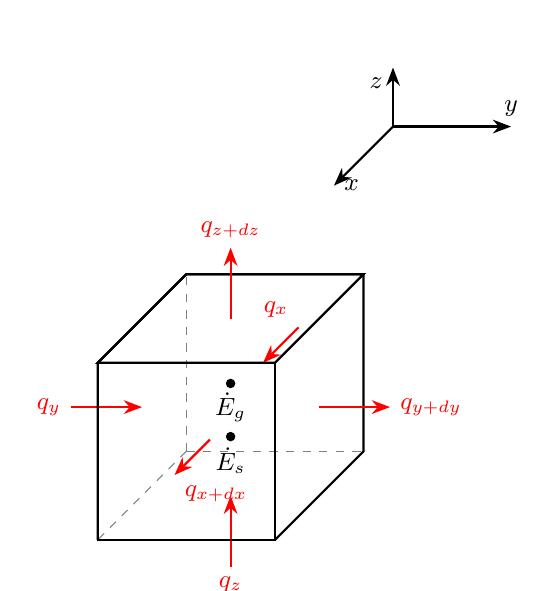
\begin{tikzpicture}[
            x={(-0.5cm,-0.5cm)}, 
            y={(1cm,0cm)}, 
            z={(0cm,1cm)}, 
            scale=1.5,
            >=Stealth,
            font=\small
        ]

            % --- Definitions ---
            \def\dx{1.5}
            \def\dy{1.5}
            \def\dz{1.5}

            % --- Coordinates ---
            \coordinate (A) at (0,0,0);
            \coordinate (B) at (\dx,0,0);
            \coordinate (C) at (\dx,\dy,0);
            \coordinate (D) at (0,\dy,0);
            
            \coordinate (E) at (0,0,\dz);
            \coordinate (F) at (\dx,0,\dz);
            \coordinate (G) at (\dx,\dy,\dz);
            \coordinate (H) at (0,\dy,\dz);

            

            % --- 1. Hidden Edges ---
            \draw[dashed, gray] (A) -- (B);
            \draw[dashed, gray] (A) -- (D);
            \draw[dashed, gray] (A) -- (E);

           

            % --- 2. Heat Inflows (Red Arrows) ---
            \draw[->, thick, red] (0.5*\dx, -0.6, 0.5*\dz) -- (0.5*\dx, 0, 0.5*\dz) node[left, pos=0] {$q_y$};
            \draw[->, thick, red] (0.5*\dx, 0.5*\dy, -0.6) -- (0.5*\dx, 0.5*\dy, 0) node[below, pos=0] {$q_z$};
            \draw[->, thick, red] (-0.6, \dy/2-0.1, \dz/2) -- (0, \dy/2-0.1, \dz/2) node[above left, pos=0] {$q_x$};

            % --- 3. Visible Cube Edges ---
            \draw[thick] (B) -- (C) -- (G) -- (F) -- cycle; 
            \draw[thick] (E) -- (F) -- (G) -- (H) -- cycle;
            \draw[thick] (E) -- (H) -- (D) -- (C); 
            \draw[thick] (E) -- (F) -- (B); 

            % --- 4. Heat Outflows ---
            \draw[->, thick, red] (\dx, \dy/2+0.2, \dz/2+0.1) -- (\dx+0.6, \dy/2+0.2, \dz/2+0.1) node[below right] {$q_{x+dx}$};
            \draw[->, thick, red] (\dx/2, \dy, \dz/2) -- (\dx/2, \dy+0.6, \dz/2) node[right] {$q_{y+dy}$};
            \draw[->, thick, red] (\dx/2, \dy/2, \dz) -- (\dx/2, \dy/2, \dz+0.6) node[above] {$q_{z+dz}$};

            % --- 5. Energy Generation & Storage ---
            \node[align=center] at (\dx/2, \dy/2, \dz/2) {$\dot{E}_{g}$};
            \filldraw[black] (\dx/2 , \dy/2, \dz/2 + .2) circle (1pt);

            \node[align=center] at (\dx/2, \dy/2, \dz/2 - 0.45) {$\dot{E}_{s}$};
            \filldraw[black] (\dx/2 , \dy/2, \dz/2 - 0.45 + .2) circle (1pt);

            % --- 6. Axes Reference ---
            \draw[->, thick, black] (-0.5, 1.5, 2.5) -- (0.5, 1.5, 2.5) node[right] {$x$};
            \draw[->, thick, black] (-0.5, 1.5, 2.5) -- (-0.5, 2.5, 2.5) node[above] {$y$};
            \draw[->, thick, black] (-0.5, 1.5, 2.5) -- (-0.5, 1.5, 3.0) node[below left] {$z$};

        \end{tikzpicture}
        \caption{Differential Control Volume.} 
        \label{fig:diff_vol}
    \end{minipage}
\end{figure}

\noindent \hfill 
\begin{minipage}{8cm} 
    \centering 
    
    \textbf{Taylor Series Expansions:}
    \begin{align*}
        q_{x+dx} &= q_x+\frac{\partial q_x}{\partial x}dx\\
        q_{y+dy} &= q_y+\frac{\partial q_y}{\partial y}dy\\
        q_{z+dz} &= q_z+\frac{\partial q_z}{\partial z}dz
    \end{align*}

    \textbf{Energy Generation:}
    \begin{align*}
        \dot{E}_{g} &= \dot{q}dxdydz
    \end{align*}

    \textbf{Energy Storage:}
    \begin{align*}
        \dot{E}_{st} &= \rho C_p\frac{\partial T}{\partial t}dxdydz
    \end{align*}

    \textbf{Conservation of Energy:}
    \begin{align*}
        \dot{E}_{in}&+\dot{E}_{g}-\dot{E}_{out} = \dot{E}_{st}\\
        (q_x+q_y+q_z)&+\dot{E}_{g}-(q_{x+dx}+q_{y+dy}+q_{z+dz})=\dot{E}_{st}
    \end{align*}
    
    \textit{Applying this and doing some algebra will get you the general heat equation.}
\end{minipage}

\clearpage

\subsection*{General Heat Eq}
\begin{align*}
    \frac{\partial}{\partial x}\Bigg(k\frac{\partial T}{\partial x}\Bigg) + \frac{\partial}{\partial y}\Bigg(k\frac{\partial T}{\partial y}\Bigg) + \frac{\partial}{\partial z}\Bigg(k\frac{\partial T}{\partial z}\Bigg) + \dot{q} &= \rho C_p \frac{\partial T}{\partial t}
\end{align*}

\subsection*{1D Conduction}

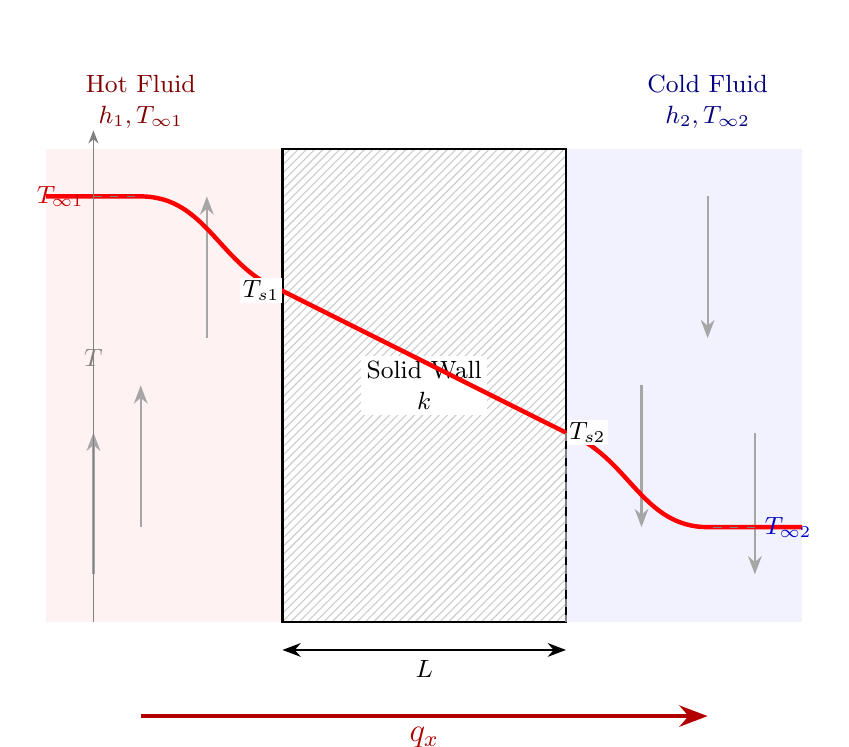
\begin{tikzpicture}[
    >=Stealth,
    font=\small,
    scale=1.2 % Adjust overall size
]

    % === DEFINITIONS & COORDINATES ===
    % Wall dimensions
    \def\wallW{3}   % Width of the wall
    \def\wallH{5}   % Height of the drawing area
    \def\blW{1.5}   % Approx width of thermal boundary layer for visualization

    % Temperature Heights (Y-coordinates to represent values)
    % T_inf1 > T_s1 > T_s2 > T_inf2
    \def\yTinfOne{4.5}
    \def\yTsOne{3.5}
    \def\yTsTwo{2.0}
    \def\yTinfTwo{1.0}

    % X-Coordinates for interfaces
    \coordinate (LeftFluidEnd) at (-\blW - 1, 0);
    \coordinate (WallStart) at (0, 0);
    \coordinate (WallEnd) at (\wallW, 0);
    \coordinate (RightFluidStart) at (\wallW + \blW + 1, 0);


    % === 1. FLUID REGIONS (Visual fluff) ===
    % Hot Fluid (Left) - faint red background tint
    \fill[red!5] (LeftFluidEnd |- 0,\wallH) rectangle (WallStart |- 0,0);
    % Cold Fluid (Right) - faint blue background tint
    \fill[blue!5] (WallEnd |- 0,\wallH) rectangle (RightFluidStart |- 0,0);

    % Fluid motion arrows (squiggly) to imply convection
    \begin{scope}[decorate, decoration={snake, amplitude=.4mm, segment length=2mm, post length=1mm}, gray!70, ->, thick]
        % Left side (Hot)
        \draw (-1.5, 1) -- (-1.5, 2.5);
        \draw (-0.8, 3) -- (-0.8, 4.5);
        \draw (-2.0, 0.5) -- (-2.0, 2);
        % Right side (Cold)
        \draw (\wallW+0.8, 2.5) -- (\wallW+0.8, 1);
        \draw (\wallW+1.5, 4.5) -- (\wallW+1.5, 3);
        \draw (\wallW+2.0, 2) -- (\wallW+2.0, 0.5);
    \end{scope}


    % === 2. THE SOLID WALL (Conduction Zone) ===
    % Draw the rectangle with a pattern
    \draw[thick, pattern=north east lines, pattern color=gray!40] 
        (WallStart) rectangle (WallEnd |- 0,\wallH);
    
    % Mark the wall thickness L
    \draw[<->, thick] ($(WallStart)+(0,-0.3)$) -- node[below] {$L$} ($(WallEnd)+(0,-0.3)$);
    
    % Label Wall properties
    \node[align=center, fill=white, inner sep=2pt] at (\wallW/2, \wallH/2) {Solid Wall\\ $k$};


    % === 3. REGION LABELS & PROPERTIES ===
    % Left Fluid
    \node[align=center, red!50!black] at (-1.5, \wallH + 0.5) {Hot Fluid\\ $h_1, T_{\infty 1}$};
    % Right Fluid
    \node[align=center, blue!50!black] at (\wallW + 1.5, \wallH + 0.5) {Cold Fluid\\ $h_2, T_{\infty 2}$};


    % === 4. THE TEMPERATURE PROFILE (The most important part) ===
    \draw[red, ultra thick] 
        % --- Hot Convection Side ---
        % Start deep in bulk fluid (constant T)
        ($(LeftFluidEnd)+(0,\yTinfOne)$) -- ($(WallStart)+(-\blW,\yTinfOne)$)
        % Boundary layer curve down to surface Ts1.
        % Using 'out' and 'in' angles creates a smooth curve representing the thermal boundary layer
        to[out=0, in=160] (WallStart |- 0, \yTsOne) coordinate (TS1)
        
        % --- Solid Conduction Side ---
        % Linear drop through the solid
        -- (WallEnd |- 0, \yTsTwo) coordinate (TS2)
        
        % --- Cold Convection Side ---
        % Boundary layer curve down from surface Ts2
        to[out=-20, in=180] ($(WallEnd)+(\blW,\yTinfTwo)$)
        % End deep in bulk fluid (constant T)
        -- ($(RightFluidStart)+(0,\yTinfTwo)$);


    % === 5. TEMPERATURE LABELS & AXES ===
    % Draw a faint y-axis for reference
    \draw[->, gray, thin] ($(LeftFluidEnd)+(0.5,0)$) -- node[above]{$T$} ($(LeftFluidEnd)+(0.5,\wallH+0.2)$);

    % Label T_inf1
    \draw[gray, dashed] ($(LeftFluidEnd)+(0.5,\yTinfOne)$) -- (-\blW, \yTinfOne);
    \node[left, red!80!black] at ($(LeftFluidEnd)+(0.5,\yTinfOne)$) {$T_{\infty 1}$};

    % Label T_s1 (Surface 1)
    \draw[gray, dashed] (TS1) -- (TS1 -| 0,0); % Drop line to x-axis
    \node[left, fill=white, inner sep=1pt] at (TS1) {$T_{s1}$};

    % Label T_s2 (Surface 2)
    \draw[gray, dashed] (TS2) -- (TS2 |- 0,0); % Drop line to x-axis
    \node[right, fill=white, inner sep=1pt] at (TS2) {$T_{s2}$};

    % Label T_inf2
    \draw[gray, dashed] ($(RightFluidStart)+(-0.5,\yTinfTwo)$) -- (\wallW+\blW, \yTinfTwo);
    \node[right, blue!80!black] at ($(RightFluidStart)+(-0.5,\yTinfTwo)$) {$T_{\infty 2}$};


    % === 6. OVERALL HEAT FLUX ARROW ===
    \draw[->, ultra thick, red!70!black] 
        (-\blW, \wallH/2 - 3.5) -- node[below, font=\large] {$q_x$} (\wallW+\blW, \wallH/2 - 3.5);

\end{tikzpicture}

\subsection*{Finding the heat xfer rate:}

\begin{enumerate}
    \item Start with the conditions in the wall.
    \item Solve the general heat equation with the appropriate boundary conditions to find temp distribution.
    \item Find the conduction Q xfer rate 
\end{enumerate}

\subsection*{Lets start with the general heat equation}

\begin{align*}
    \frac{\partial}{\partial x}\Bigg(k\frac{\partial T}{\partial x}\Bigg) + \frac{\partial}{\partial y}\Bigg(k\frac{\partial T}{\partial y}\Bigg) + \frac{\partial}{\partial z}\Bigg(k\frac{\partial T}{\partial z}\Bigg) + \dot{q} &= \rho C_p \frac{\partial T}{\partial t}
\end{align*}




For our 1D wall with no heat source and steady state, this reduces to:


\begin{align*}
    \frac{d}{dx}\Bigg(k\frac{dT}{dx}\Bigg)&=0
\end{align*}

We will solve this to find $T(x)$ or "Temp Distribution"

Assume k is constant through the wall.

\begin{align*}
    \int\frac{d}{dx}\Bigg(k\frac{dT}{dx}\Bigg)dx&=\int 0 dx\\
    k\frac{dT}{dx}&= A\\
    \frac{dT}{dx}&=\frac{A}{k}\\
    \frac{dT}{dx}&=C_1 \quad\quad \text{where $C_1 = \frac{A}{k}$}\\
    dT&=C_1dx\\
    \int dT dx&=\int C_1 dx\\
    T(x)&=C_1x+C_2\\
\end{align*}
What about non-constant k terms?

\begin{align*}
\frac{d}{dx}(k(t)\frac{dT}{dx})&=0\\
\int \frac{d}{dx}k(t)\frac{dT}{dx}dx&=\int 0 dx\\
k(T)\frac{dT}{dx}&=\tikzmarknode{C0}{C_0}\\
k(T) dT &= C_0 dx\\
\int k(T) dT&= \int C_0 dx\\
\int k_0(1+\beta T) dT&= \int C_0 dx\\
k_0\int (1+\beta T) dT&= C_0x+C_1\\
k_0\Bigg[T+\frac{\beta T^2}{2}\Bigg]&= C_0x+C_1 \\
x(t)&=\frac{T+\frac{\beta}{2}T^2}{1+\frac{\beta}{2}} \tag{plotted below}
\end{align*}



\begin{tikzpicture}[remember picture, overlay]
    \draw[<-, thick, blue] (C0) -- ++(2cm, 0) node[right] {Still Constant flux};
\end{tikzpicture}

\begin{figure}[H]
    \centering
    
\includegraphics[width=0.75\linewidth]{Unit 3/betaComp.jpg}
    \caption{with BC $T(x=0)=0$ and $T(x=L)=T_s$}
    \label{fig:placeholder}
\end{figure}

\subsection{numerical view of the work}

\begin{center}
    \begin{eqnbox}
        $\displaystyle \frac{d}{dx}\left( k \frac{dT}{dx} \right) = 0$
    \end{eqnbox}
\end{center}


So with the $T(x)$ that we found, we can see that we still need the constants. Lets get those:

\begin{align*}
    T(x)&=C_1x+C_2\\
    \intertext{Apply the boundary conditions}\\
    \intertext{$T(x=0)=T_{s1}$ and $T(x=L)=T_{s2}$}\\
    T(x=0)& \quad \textbf{First}\\
    T(x=0)&=C_1(x=0)+C_2\\
    T_{s1}&=C_10+C_2\\
    T_{s1}&=\tikzmarknode{c2E}{C_2}
\end{align*}

\begin{align*}
    T(x=L)& \quad \textbf{Second}\\
    T(x=L)&=C_1(x=L)+C_2\\
    T_{s2}&=C_1L+\tikzmarknode{c2S}{T_{s1}}\\
    C_1&=\frac{T_{s2}-T_{s1}}{L}
\end{align*}

with $C_1$ and $C_2$ we can finsish T(x):


\begin{center}
    \begin{eqnbox}
        $\displaystyle 
        T(x) = \frac{T_{s2}-T_{s1}}{L}x + T_{s1}
        \qquad % Adds a nice horizontal gap
        \begin{aligned}
            & \text{1. 1D} \\
            & \text{2. Steady State} \\
            & \text{3. No Source/Sink}\\
            & \text{4. k is constant}
        \end{aligned}
        $
    \end{eqnbox}
\end{center}

\subsection*{Find Conduction Heat transfer}
Now that we have $T(x)$ "the temp distr WRT x"\\
we can now move to conduction heat xfer rate.

\begin{align*}
 T(x) &= \frac{T_{s2}-T_{s1}}{L}x + T_{s1}\\
 \intertext{Apply Fourier's Law}\\
 q_{x}&=-kA_{\perp}\frac{dT}{dn}\\
 q_{x}&=-kA_{\perp}\frac{d}{dx}\Bigg[\frac{T_{s2}-T_{s1}}{L}x + T_{s1} \Bigg]\\
 q_{x} &= -kA_{\perp}\frac{T_{s2}-T_{s1}}{L}\frac{d}{dx} x + \canceldown{0}{\frac{d}{dx} T_{s1}}\\
 q_{x} &= \frac{-kA_{\perp}}{L}(T_{s2}-T_{s1})\\
\end{align*}

\begin{figure}[H]
    \hfill
    \begin{minipage}{8cm} 
        \centering        
        
        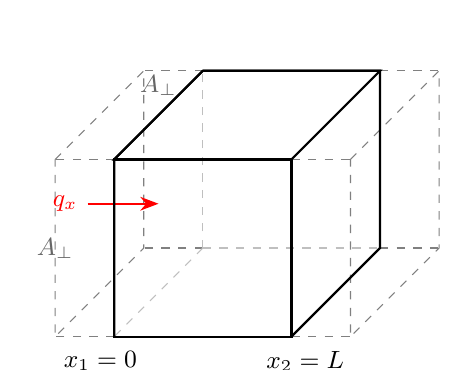
\begin{tikzpicture}[
            x={(-0.5cm,-0.5cm)}, 
            y={(1cm,0cm)}, 
            z={(0cm,1cm)}, 
            scale=1.5,
            >=Stealth,
            font=\small
        ]

            % --- Definitions ---
            \def\dx{1.5}
            \def\dy{1.5}
            \def\dz{1.5}
            \def\offset{0.5} % How far the dashed lines extend

            % --- Cube Coordinates ---
            \coordinate (A) at (0,0,0);
            \coordinate (B) at (\dx,0,0);
            \coordinate (C) at (\dx,\dy,0);
            \coordinate (D) at (0,\dy,0);
            
            \coordinate (E) at (0,0,\dz);
            \coordinate (F) at (\dx,0,\dz);
            \coordinate (G) at (\dx,\dy,\dz);
            \coordinate (H) at (0,\dy,\dz);

            % --- LEFT Side Extensions (y = -0.5) ---
            \coordinate (L1) at (\dx, -\offset, \dz); % Top-Front
            \coordinate (L2) at (0,   -\offset, \dz); % Top-Back
            \coordinate (L3) at (\dx, -\offset, 0);   % Bottom-Front
            \coordinate (L4) at (0,   -\offset, 0);   % Bottom-Back

            % --- RIGHT Side Extensions (y = dy + 0.5) ---
            \coordinate (R1) at (\dx, \dy+\offset, \dz); % Top-Front
            \coordinate (R2) at (0,   \dy+\offset, \dz); % Top-Back
            \coordinate (R3) at (\dx, \dy+\offset, 0);   % Bottom-Front
            \coordinate (R4) at (0,   \dy+\offset, 0);   % Bottom-Back


            % --- 1. Draw Left Extension (Ghost Face) ---
            \draw[dashed, gray] (F) -- (L1);
            \draw[dashed, gray] (E) -- (L2);
            \draw[dashed, gray] (B) -- (L3);
            \draw[dashed, gray] (A) -- (L4);
            % Draw the Ghost Face itself
            \draw[dashed, gray] (L1) -- (L2) -- (L4) -- (L3) -- cycle;
            % Label A_perp
            \node[gray!80!black] at (\dx, -\offset, 0.5*\dz) {$A_{\perp}$};


            % --- 2. Draw Right Extension (Ghost Face) ---
            \draw[dashed, gray] (G) -- (R1);
            \draw[dashed, gray] (H) -- (R2);
            \draw[dashed, gray] (C) -- (R3);
            \draw[dashed, gray] (D) -- (R4);
            % Draw the Ghost Face itself
            \draw[dashed, gray] (R1) -- (R2) -- (R4) -- (R3) -- cycle;
            % Label A_perp
            \node[gray!80!black] at (0.25,-0.25,\dz) {$A_{\perp}$};


            % --- 3. Hidden Cube Edges ---
            \draw[dashed, gray!50] (A) -- (B);
            \draw[dashed, gray!50] (A) -- (D);
            \draw[dashed, gray!50] (A) -- (E);

            % --- 4. Heat Inflows (Red Arrows) ---
            \draw[->, thick, red] (0.5*\dx, -0.6, 0.5*\dz) -- (0.5*\dx, 0, 0.5*\dz) node[left, pos=0] {$q_x$};

            % --- 5. Visible Cube Edges ---
            \draw[thick] (B) -- (C) -- (G) -- (F) -- cycle; 
            \draw[thick] (E) -- (F) -- (G) -- (H) -- cycle;
            \draw[thick] (E) -- (H) -- (D) -- (C); 
            \draw[thick] (E) -- (F) -- (B); 

            % --- 6. LABELS ADDED HERE ---
            % Positioned slightly below the corners B and C
            \node[below, xshift=-5pt, yshift=-2pt] at (B) {$x_1=0$};
            \node[below, xshift=5pt, yshift=-2pt]  at (C) {$x_2=L$};

        \end{tikzpicture}
        \caption{This shows the normal area $A_{\perp}$ is normal to the heat.} 
        \label{fig:diff_vol}
    \end{minipage}
\end{figure}

\subsection*{Find Heat Flux Rate}
\begin{align*}
    q_x''&=\frac{Q_x}{A}\\
    &=\frac{\frac{-kA_{\perp}}{L}(T_{s2}-T_{s1})}{A}\\
    q_x''&=\frac{-k}{L}(T_{s2}-T_{s1})
\end{align*}

\subsection*{3.1.2 - Thermal Resistance}
First, some circuit stuff

\subsection*{3.1.2 - Thermal Resistance}
First, some circuit stuff. There is a direct analogy between the flow of electricity and the flow of heat.

\begin{center}
    \renewcommand{\arraystretch}{1.5}
    \begin{tabular}{c | c }
        \textbf{Electrical System} & \textbf{Thermal System} \\
        \hline
        Current flow, $I$ [Amps] & Heat transfer rate, $q_x$ [Watts] \\
        Voltage potential, $\Delta V$ [Volts] & Temperature difference, $\Delta T$ [K] \\
        Electrical Resistance, $R_e$ [$\Omega$] & Thermal Resistance, $R_{th}$ [K/W] \\
        \hline
        \textbf{Ohm's Law:} $\displaystyle I = \frac{\Delta V}{R_e}$ & \textbf{Fourier's Law:} $\displaystyle q_x = \frac{\Delta T}{R_{th}}$
    \end{tabular}
\end{center}

\noindent Based on this analogy, we can define the \textbf{Conduction Resistance} for a plane wall. 
From our previous equation for heat rate:

\begin{align*}
    q_x &= \frac{kA}{L}(T_{s1} - T_{s2}) \\
    q_x &= \frac{T_{s1} - T_{s2}}{\left( \frac{L}{kA} \right)}
\end{align*}

\noindent \textbf{Note on Sign Convention:}\\ 
You might expect to see $\Delta T = T_{final} - T_{initial}$ ($T_{s2} - T_{s1}$). However, heat transfer always flows from \textbf{High Temp} to \textbf{Low Temp}. 

Fourier's Law includes a negative sign ($q = -k \dots$) to correct for this natural gradient. In the resistance analogy, we simplify this by defining the driving potential as:
\[
    \text{Potential} = T_{high} - T_{low} = T_{s1} - T_{s2}
\]
This ensures our heat rate $q_x$ is a positive value flowing in the direction of the arrow, exactly like Voltage Drop ($V_{high} - V_{low}$) in a circuit.
\\
\\
Comparing this to the "Thermal Ohm's Law" ($q = \Delta T / R$), the denominator represents the resistance:

\begin{center}
    \begin{eqnbox}
        $\displaystyle R_{t, cond} = \frac{T_{s1}-T_{s2}}{q_x} = \frac{L}{kA}$
    \end{eqnbox}
    \footnotesize\textit{(Thermal Resistance for Plane Wall Conduction)}
\end{center}

\subsubsection*{The Thermal Circuit}
We can now draw the wall as a resistor between two temperature nodes:

\begin{center}
\begin{circuitikz}[scale=1.2, transform shape]
    \draw 
    (0,0) node[label={above:$T_{s1}$}, circle, fill, inner sep=2pt] (A) {}
    to[R, l=$R_{cond} {=} \frac{L}{kA}$] (4,0) 
    node[label={above:$T_{s2}$}, circle, fill, inner sep=2pt] (B) {};
    
    \draw[->, thick, red] (0.5, -0.6) -- node[below] {$q_x$} (3.5, -0.6);
\end{circuitikz}
\end{center}

\textbf{What about convection?}

Using Newtons law of cooling
\begin{align*}
    q&=hA(T_s-T_{\infty})\\
    \frac{T_s-T_{\infty}}{q}&=\frac{1}{hA}
\end{align*}

\begin{center}
    \begin{eqnbox}
        $\displaystyle R_{conv}=\frac{T_s-T_{\infty}}{q}=\frac{1}{hA}$
    \end{eqnbox}
    \footnotesize\textit{(convective resistance, High to low)}
\end{center}
\subsection*{The equivalent thermal circuit}

\begin{figure}[H]
    \centering
    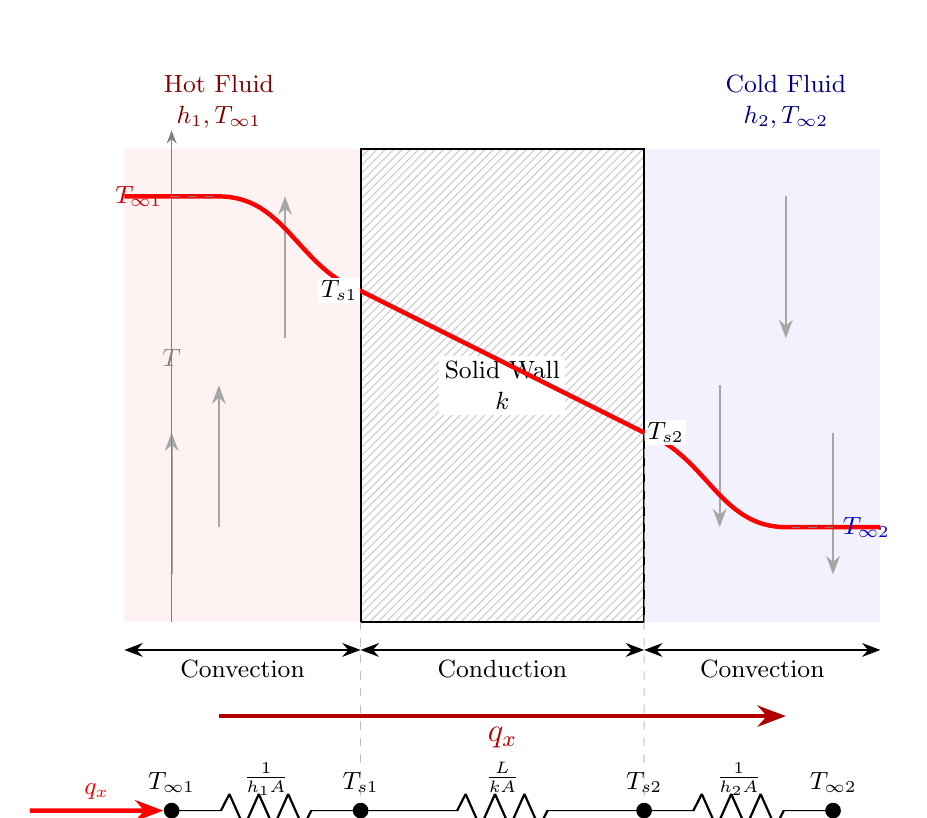
\begin{tikzpicture}[
        >=Stealth,
        font=\small,
        scale=1.2
    ]

        % === DEFINITIONS & COORDINATES ===
        \def\wallW{3}   % Width of the wall
        \def\wallH{5}   % Height of the drawing area
        \def\blW{1.5}   % Approx width of thermal boundary layer

        % Temperature Heights
        \def\yTinfOne{4.5}
        \def\yTsOne{3.5}
        \def\yTsTwo{2.0}
        \def\yTinfTwo{1.0}

        % X-Coordinates
        \coordinate (LeftFluidEnd) at (-\blW - 1, 0);
        \coordinate (WallStart) at (0, 0);
        \coordinate (WallEnd) at (\wallW, 0);
        \coordinate (RightFluidStart) at (\wallW + \blW + 1, 0);

        % === 1. FLUID REGIONS ===
        \fill[red!5] (LeftFluidEnd |- 0,\wallH) rectangle (WallStart |- 0,0);
        \fill[blue!5] (WallEnd |- 0,\wallH) rectangle (RightFluidStart |- 0,0);

        % Fluid motion arrows
        \begin{scope}[decorate, decoration={snake, amplitude=.4mm, segment length=2mm, post length=1mm}, gray!70, ->, thick]
            \draw (-1.5, 1) -- (-1.5, 2.5);
            \draw (-0.8, 3) -- (-0.8, 4.5);
            \draw (-2.0, 0.5) -- (-2.0, 2);
            \draw (\wallW+0.8, 2.5) -- (\wallW+0.8, 1);
            \draw (\wallW+1.5, 4.5) -- (\wallW+1.5, 3);
            \draw (\wallW+2.0, 2) -- (\wallW+2.0, 0.5);
        \end{scope}

        % === 2. THE SOLID WALL & LABELS ===
        \draw[thick, pattern=north east lines, pattern color=gray!40] 
            (WallStart) rectangle (WallEnd |- 0,\wallH);
        
        \draw[<->, thick] ($(LeftFluidEnd)+(0,-0.3)$) -- node[below] {Convection} ($(WallStart)+(0,-0.3)$);
        \draw[<->, thick] ($(WallStart)+(0,-0.3)$) -- node[below] {Conduction} ($(WallEnd)+(0,-0.3)$);
        \draw[<->, thick] ($(WallEnd)+(0,-0.3)$) -- node[below] {Convection} ($(RightFluidStart)+(0,-0.3)$);
        
        \node[align=center, fill=white, inner sep=2pt] at (\wallW/2, \wallH/2) {Solid Wall\\ $k$};

        % === 3. REGION LABELS ===
        \node[align=center, red!50!black] at (-1.5, \wallH + 0.5) {Hot Fluid\\ $h_1, T_{\infty 1}$};
        \node[align=center, blue!50!black] at (\wallW + 1.5, \wallH + 0.5) {Cold Fluid\\ $h_2, T_{\infty 2}$};

        % === 4. TEMPERATURE PROFILE ===
        \draw[red, ultra thick] 
            ($(LeftFluidEnd)+(0,\yTinfOne)$) -- ($(WallStart)+(-\blW,\yTinfOne)$)
            to[out=0, in=160] (WallStart |- 0, \yTsOne) coordinate (TS1)
            -- (WallEnd |- 0, \yTsTwo) coordinate (TS2)
            to[out=-20, in=180] ($(WallEnd)+(\blW,\yTinfTwo)$)
            -- ($(RightFluidStart)+(0,\yTinfTwo)$);

        % === 5. LABELS & AXES ===
        \draw[->, gray, thin] ($(LeftFluidEnd)+(0.5,0)$) -- node[above]{$T$} ($(LeftFluidEnd)+(0.5,\wallH+0.2)$);
        
        % Temperature Labels
        \draw[gray, dashed] ($(LeftFluidEnd)+(0.5,\yTinfOne)$) -- (-\blW, \yTinfOne);
        \node[left, red!80!black] at ($(LeftFluidEnd)+(0.5,\yTinfOne)$) {$T_{\infty 1}$};
        \draw[gray, dashed] (TS1) -- (TS1 -| 0,0);
        \node[left, fill=white, inner sep=1pt] at (TS1) {$T_{s1}$};
        \draw[gray, dashed] (TS2) -- (TS2 |- 0,0);
        \node[right, fill=white, inner sep=1pt] at (TS2) {$T_{s2}$};
        \draw[gray, dashed] ($(RightFluidStart)+(-0.5,\yTinfTwo)$) -- (\wallW+\blW, \yTinfTwo);
        \node[right, blue!80!black] at ($(RightFluidStart)+(-0.5,\yTinfTwo)$) {$T_{\infty 2}$};

        % === 6. HEAT FLUX ARROW (Main Diagram) ===
        \draw[->, ultra thick, red!70!black] 
            (-\blW, \wallH/2 - 3.5) -- node[below, font=\large] {$q_x$} (\wallW+\blW, \wallH/2 - 3.5);

        % === 7. TOTAL EQUIV THERMAL CIRCUIT ===
        \def\yCirc{-2.0}
        
        % Draw dashed lines connecting diagram to circuit
        \draw[gray!50, dashed] (WallStart) -- (0, \yCirc);
        \draw[gray!50, dashed] (WallEnd) -- (\wallW, \yCirc);
        
        % Circuit Drawing
        \draw 
            % Node 1: T_inf1
            (-2.0, \yCirc) node[label={above:$T_{\infty 1}$}, circle, fill, inner sep=2pt] (C1) {}
            % Resistor 1: Convection
            to[R, l=$\frac{1}{h_1 A}$] (0, \yCirc) 
            % Node 2: Ts1
            node[label={above:$T_{s1}$}, circle, fill, inner sep=2pt] (C2) {}
            % Resistor 2: Conduction
            to[R, l=$\frac{L}{kA}$] (\wallW, \yCirc) 
            % Node 3: Ts2
            node[label={above:$T_{s2}$}, circle, fill, inner sep=2pt] (C3) {}
            % Resistor 3: Convection
            to[R, l=$\frac{1}{h_2 A}$] (\wallW + 2.0, \yCirc) 
            % Node 4: T_inf2
            node[label={above:$T_{\infty 2}$}, circle, fill, inner sep=2pt] (C4) {};
            
        % --- ADDED: Heat Flux Input Arrow into First Node ---
        \draw[->, ultra thick, red] 
            ($(C1) + (-1.5, 0)$) -- node[above] {$q_x$} (C1);

    \end{tikzpicture}
    \caption{Temperature distribution and equivalent thermal circuit.}
\end{figure}
\begin{align*}
        q_x = \frac{T_{\infty}-T_{s1}}{\frac{1}{hA}}=\frac{T_{s1}-T_{s2}}{\frac{L}{kA}}=\frac{T_{s2}-T_{\infty}}{\frac{1}{hA}}
    \end{align*}
    Notice that we have a total $\Delta T$ limit from $T_{\infty 1}$ and $T_{\infty 2}$ and $R_{tot}$ is a sum of resistors in series.

    \begin{align*}
        R_{tot}=\frac{1}{h_1A}+\frac{L}{kA}+\frac{1}{h_2A} 
    \end{align*}
so
\begin{align*}
    q_x=\frac{T_{\infty 1}-T_{\infty 2}}{R_{tot}}
\end{align*}


    \subsection*{Block Diagram Representation}

 a control (block) diagram represents the system response
\begin{itemize}
    \item \textbf{Input:} The driving potential difference ($\Delta T$)
    \item \textbf{System Gain:} The total thermal conductance ($1/R_{tot}$)
    \item \textbf{Output:} The resulting heat flow ($q_x$)
\end{itemize}

\begin{center}
\begin{tikzpicture}[auto, node distance=2cm, >=latex']
    % Define block styles
    \tikzstyle{block} = [draw, rectangle, minimum height=3em, minimum width=4em]
    \tikzstyle{sum} = [draw, circle, node distance=1cm]
    \tikzstyle{input} = [coordinate]
    \tikzstyle{output} = [coordinate]

    % --- Nodes ---
    \node [input] (input1) {};
    \node [sum, right of=input1] (sum) {$\Sigma$};
    \node [input, below of=sum, node distance=1.5cm] (input2) {};
    \node [block, right of=sum, node distance=3.5cm] (system) {$\displaystyle \frac{1}{R_{tot}}$};
    \node [output, right of=system, node distance=2cm] (output) {};

    % --- Edges ---
    % T_inf1 into Sum
    \draw [->, thick] (input1) -- node {$T_{\infty 1}$} node[pos=0.9, below] {$+$} (sum);
    
    % T_inf2 into Sum (Negative feedback style)
    \draw [->, thick] (input2) -- node [right] {$T_{\infty 2}$} node[pos=0.9, right] {$-$} (sum);
    
    % Delta T into System
    \draw [->, thick] (sum) -- node {$\Delta T_{total}$} (system);
    
    % q_x out of System
    \draw [->, thick] (system) -- node [name=y] {$q_x$} (output);

\end{tikzpicture}
\end{center}

\noindent This helps visualize that heat transfer is a linear system where the flow $q_x$ is directly proportional to the temperature difference, scaled by the system's "Conductance" ($UA = 1/R_{tot}$).


\end{document}